% !TEX program = lualatex
\documentclass[12pt,a4paper]{article}
\usepackage{amsmath,amssymb,amsthm}
\usepackage{geometry}
\geometry{margin=2.5cm}
\usepackage{hyperref}
\hypersetup{colorlinks=true,linkcolor=blue,citecolor=blue,urlcolor=blue}
\usepackage{booktabs}
\usepackage{lmodern}
\usepackage[T1]{fontenc}
\usepackage{graphicx}

\title{Realization of Simple Harmonic Oscillation and Sinusoidal Waves\\
in the Delay Circuit Model}

\author{Noriaki Kihara\\
WF System Co., Ltd.\\
Osaka University, School of Engineering Science (graduated)}

\date{April 2026\quad Research Note\\[4pt]
DOI: \href{https://doi.org/10.5281/zenodo.19534349}{10.5281/zenodo.19534349}}

\begin{document}

\maketitle

\begin{abstract}
The delay circuit model constructed in the previous paper~\cite{ref1} could only express
square wave oscillation, because it used only the class $A = \{I, \overline{I}\}$ and the
inversion (NOT) operation. In this paper, using the framework of superclasses,
meta-information, and the operation function $*$ introduced in the previous paper~\cite{ref2},
we realize sinusoidal waves (transverse waves), longitudinal waves, and rotational waves by
concretely defining the class information and the $*$ operation. In all cases, we show that
different wave patterns can be obtained solely by the choice of class definition and operation
function $*$, without modifying the definitions of the delay circuit $F_D$ or the NOT operation
circuit.
\end{abstract}

\section{Introduction}

In the previous paper~\cite{ref1}, we constructed discrete square wave oscillation using only
the class $A = \{I, \overline{I}\}$ and the inversion (NOT) operation. In the previous
paper~\cite{ref2}, we introduced superclasses, meta-information (counter $n$, operation
function $*$), and an extended definition of $F_D$.

In this paper, using the framework of~\cite{ref2}, we construct models that realize sinusoidal
waves (longitudinal waves, transverse waves, and rotational waves) by concretely defining the
class $A$ information, meta-information, and operation function $*$.

\section{Preparation: Summary of Definitions from Previous Papers}

This paper presupposes the delay circuit $F_D$, the NOT operation circuit, and the properties
of information $I$ (null state, equivalence judgment, inversion) defined in the previous
paper~\cite{ref1}. We also use the following concepts introduced in the previous
paper~\cite{ref2}:

\begin{itemize}
  \item \textbf{Superclass}: A tuple $(A, B, C_1, \ldots, C_m)$ of information belonging to
        different classes (\cite{ref2}~\S3.2)
  \item \textbf{Meta-information}: Counter $n$ (number of delays) and operation function $*$
        (\cite{ref2}~\S3.2)
  \item \textbf{Extended definition of $F_D$}: When passing through $F_D$, the counter $n$ is
        incremented, and $*$ is executed if it is not $\mathrm{null}$ (\cite{ref2}~\S3.3)
\end{itemize}

For the details of these definitions, refer to the respective previous papers.

\section{Definition of the Simple Harmonic Oscillation Class $A$}

\subsection{Simple Harmonic Oscillation Circuit in the Previous Paper}

In the previous paper~\cite{ref1}~\S3, a feedback structure was constructed by connecting the
delay circuit $F_D$ and the NOT operation circuit: the output of $F_D$ is connected to the
input of NOT, and the output of NOT is connected to the input of $F_D$.

\begin{figure}[h]
  \centering
  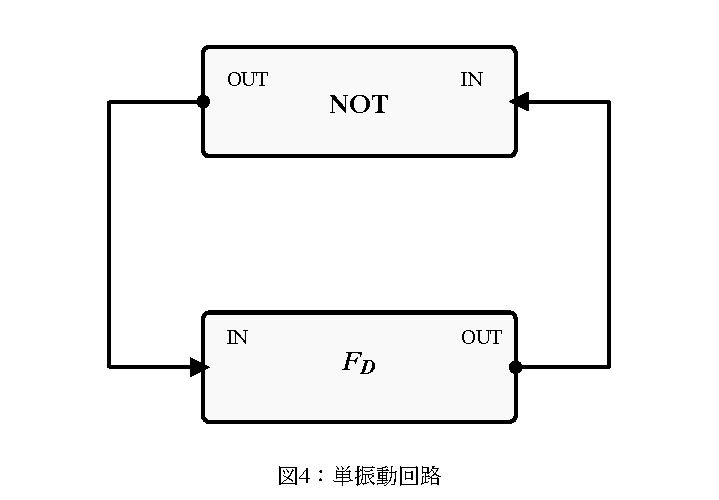
\includegraphics[width=0.6\textwidth]{fig4_oscillation_circuit.pdf}
  \caption{Simple harmonic oscillation circuit (reprinted from \cite{ref1} Figure~4)}
  \label{fig:oscillation_circuit}
\end{figure}

The output transitions of the simple harmonic oscillation circuit at each step are shown
in Table~\ref{tab:sq_wave}.

\begin{table}[h]
  \centering
  \caption{Output transitions of the simple harmonic oscillation circuit}
  \label{tab:sq_wave}
  \begin{tabular}{ccc}
    \toprule
    Number of delays $n$ & OUT of $F_D$ & OUT of NOT \\
    \midrule
    0 & $\mathrm{null}$ & $\mathrm{null}$ \\
    1 & $I$             & $\overline{I}$  \\
    2 & $\overline{I}$  & $I$             \\
    3 & $I$             & $\overline{I}$  \\
    4 & $\overline{I}$  & $I$             \\
    $\vdots$ & $\vdots$ & $\vdots$        \\
    \bottomrule
  \end{tabular}
\end{table}

For $n \geq 1$, the output of $F_D$ alternates between $I$ and $\overline{I}$. This is a
discrete oscillation.

Taking information $I$ as a scalar value and defining inversion as $\overline{I} = -I$, the
output of $F_D$ in the simple harmonic oscillation circuit is expressed as follows:

\begin{equation}
  x(n) = I \cdot (-1)^{n+1} \quad (n = 1, 2, 3, \ldots)
\end{equation}

That is, the output alternates between $I$ and $-I$ with respect to the number of delays $n$.
This is a square wave.

\subsection{Definition of the Square Wave Class $A$}

In the framework of the previous paper~\cite{ref2}, we redefine the square wave oscillation
of \S3.1.

\begin{itemize}
  \item \textbf{Class $A$ information}: Scalar value $i$
  \item \textbf{Meta-information}: $\mathrm{null}$ (neither the counter $n$ nor the operation
        function $*$ is required)
\end{itemize}

Inversion is given as $\overline{i} = -i$ by the NOT operation circuit. Since the
meta-information is $\mathrm{null}$, no additional operation is performed when passing through
$F_D$, and the same result as the simple harmonic oscillation circuit of \S3.1 is obtained.

\begin{equation}
  x(n) = i \cdot (-1)^{n+1} \quad (n = 1, 2, 3, \ldots)
\end{equation}

\subsection{Propagation and Oscillation via the Square Wave Class $A$}

We apply the square wave class $A$ defined in \S3.2 (scalar value $i$, meta-information
$\mathrm{null}$) to the open rope model of the previous paper~\cite{ref1}~\S4 and the closed
rope model of~\cite{ref1}~\S5.

Since the meta-information is $\mathrm{null}$, no additional operation is performed when
passing through $F_D$. Only the basic operation rule of $F_D$ (copying the input information
internally and outputting it after a delay of one step) operates.

Therefore, in the open rope model, information $i$ passes through each $F_D$ one step at a
time unchanged, giving the same propagation sequence as~\cite{ref1}~\S4 (arrival position
$k = n$). In the closed rope model, including inversion by the NOT operation circuit, the same
oscillation sequence as~\cite{ref1}~\S5 is obtained (1 oscillation $= 2n$ operations).

That is, the square wave class $A$ exactly reproduces the results of all configurations in
the previous paper~\cite{ref1} (simple harmonic oscillation circuit, open rope, closed rope).

\subsection{Definition of the Transverse Wave Class $B$}

We define class $B$ to realize a transverse wave as follows.

\textbf{Class $B$ information:}
\begin{itemize}
  \item $i$: Scalar value (input value; same as class $A$)
  \item $w$: Real value (amplitude; for output)
\end{itemize}

\textbf{Meta-information:}
\begin{itemize}
  \item $n$: Counter (number of delays; as defined in~\cite{ref2}~\S3.3)
  \item $m$: Number of delays corresponding to the wavelength (a positive integer
        $1, 2, 3, \ldots$)
\end{itemize}

\textbf{Operation function $*$:}

\begin{equation}
  w = i \cdot \sin\!\left(\frac{n}{m} \cdot 360°\right)
\end{equation}

Each time a pass through $F_D$ occurs, $n$ is incremented and the operation function $*$ is
executed to update $w$. By observing the output $w$, a sinusoidal oscillation is obtained as
the number of delays $n$ advances.

\subsection{Oscillation Sequence of Class $B$}

For $i = 1$ and $m = 12$, the transitions of the output $w$ of $F_D$ in the simple harmonic
oscillation circuit are shown in Table~\ref{tab:classB}.

\begin{table}[h]
  \centering
  \caption{Oscillation sequence of class $B$ ($i = 1$, $m = 12$)}
  \label{tab:classB}
  \begin{tabular}{ccc}
    \toprule
    Number of delays $n$ & $n/m \cdot 360°$ & $w = \sin(n/m \cdot 360°)$ \\
    \midrule
    0  & $0°$   & $0.000$  \\
    1  & $30°$  & $0.500$  \\
    2  & $60°$  & $0.866$  \\
    3  & $90°$  & $1.000$  \\
    4  & $120°$ & $0.866$  \\
    5  & $150°$ & $0.500$  \\
    6  & $180°$ & $0.000$  \\
    7  & $210°$ & $-0.500$ \\
    8  & $240°$ & $-0.866$ \\
    9  & $270°$ & $-1.000$ \\
    10 & $300°$ & $-0.866$ \\
    11 & $330°$ & $-0.500$ \\
    12 & $360°$ & $0.000$  \\
    \bottomrule
  \end{tabular}
\end{table}

One period is completed at $n = 12$, and the same pattern repeats thereafter.

\begin{figure}[h]
  \centering
  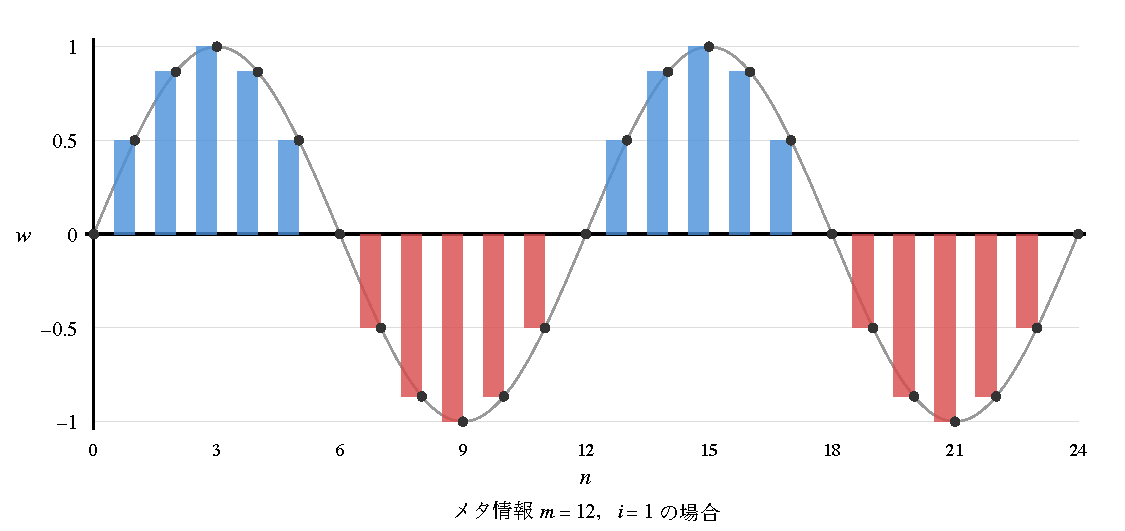
\includegraphics[width=0.75\textwidth]{fig7_sine_wave_sequence.pdf}
  \caption{Oscillation sequence of class $B$ (meta-information $m = 12$, $i = 1$).
           The bar chart shows the discrete output $w$ at each number of delays $n$,
           and the thin line shows the continuous sinusoidal wave.}
  \label{fig:classB_sequence}
\end{figure}

\section{Realization of Longitudinal Waves}

\subsection{Definition of the Longitudinal Wave Class $C$}

We define class $C$ to realize a longitudinal wave. The structure of the information,
meta-information, and operation function $*$ of class $C$ is exactly the same as that of
class $B$ (\S3.4).

\begin{itemize}
  \item \textbf{Class $C$ information}: Scalar value $i$, real value $w$
  \item \textbf{Meta-information}: Counter $n$, number of delays $m$ corresponding to the
        wavelength
  \item \textbf{Operation function $*$}: $w = i \cdot \sin(n / m \cdot 360°)$
\end{itemize}

The only difference from class $B$ is in the interpretation of the output $w$. In class $B$,
$w$ is treated as a displacement perpendicular to the direction of propagation (transverse
wave), whereas in class $C$, $w$ is treated as a \textbf{displacement in the direction of
propagation}. That is, $w$ is interpreted as the deviation of each $F_D$ from its reference
position along the horizontal axis.

\subsection{Visualization of Longitudinal Waves}

When class $C$ is applied to the open rope model, each $F_D$ is displaced by $w$ from its
reference position in the direction of propagation. As a result, regions where the bars are
dense (compression) and regions where they are sparse (rarefaction) appear alternately,
yielding the compression-rarefaction pattern of a longitudinal wave.

\begin{figure}[h]
  \centering
  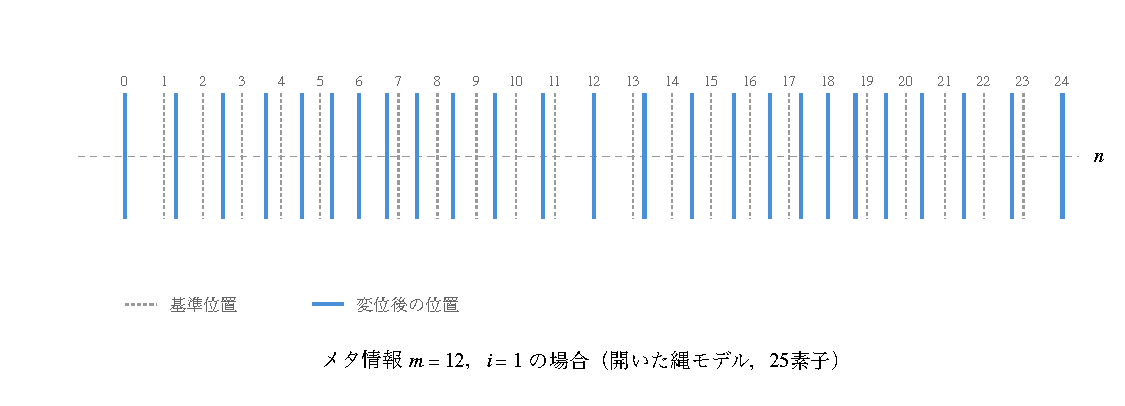
\includegraphics[width=0.75\textwidth]{fig8_longitudinal_wave.pdf}
  \caption{Compression-rarefaction pattern of a longitudinal wave by class $C$
           (meta-information $m = 12$, $i = 1$).
           Dashed lines indicate the reference positions of each $F_D$;
           solid lines indicate the positions after displacement by $w$.}
  \label{fig:longitudinal_wave}
\end{figure}

\section{Realization of Rotational Waves}

\subsection{Definition of the Rotational Wave Class $D$}

We define class $D$ to realize a rotational wave. The structure of the information and
meta-information of class $D$ is exactly the same as that of class $B$ (\S3.4).

\begin{itemize}
  \item \textbf{Class $D$ information}: Scalar value $i$, real value $w$
  \item \textbf{Meta-information}: Counter $n$, number of delays $m$ corresponding to the
        wavelength
\end{itemize}

The only differences from class $B$ are the operation function $*$ and the interpretation of
the output $w$.

\textbf{Operation function $*$:}

\begin{equation}
  w = \frac{n}{m} \cdot 360° \bmod 360°
\end{equation}

The output $w$ is interpreted as an \textbf{angle}. Each time a pass through $F_D$ occurs,
$n$ is incremented and $w$ is updated. $w$ advances from $0°$ to $360°$ in constant
increments, and returns to $0°$ upon reaching $360°$.

\subsection{Oscillation Sequence of Class $D$}

For $i = 1$ and $m = 12$, the transitions of the output $w$ (angle) of $F_D$ in the simple
harmonic oscillation circuit are shown in Table~\ref{tab:classD}.

\begin{table}[h]
  \centering
  \caption{Oscillation sequence of class $D$ ($i = 1$, $m = 12$)}
  \label{tab:classD}
  \begin{tabular}{cc}
    \toprule
    Number of delays $n$ & $w = (n/m \cdot 360°) \bmod 360°$ \\
    \midrule
    0  & $0°$   \\
    1  & $30°$  \\
    2  & $60°$  \\
    3  & $90°$  \\
    4  & $120°$ \\
    5  & $150°$ \\
    6  & $180°$ \\
    7  & $210°$ \\
    8  & $240°$ \\
    9  & $270°$ \\
    10 & $300°$ \\
    11 & $330°$ \\
    12 & $0°$   \\
    13 & $30°$  \\
    14 & $60°$  \\
    $\vdots$ & $\vdots$ \\
    \bottomrule
  \end{tabular}
\end{table}

One full rotation ($360°$) is completed at $n = 12$, and the same pattern repeats thereafter.
If the output $w$ is interpreted as an angle, this represents motion rotating at a constant
angular velocity.

\section{Conclusion}

Using the framework of superclasses, meta-information, and operation function $*$ introduced
in the previous paper~\cite{ref2}, we defined classes $B$, $C$, and $D$ to realize transverse
waves (sinusoidal waves), longitudinal waves, and rotational waves. The correspondence of each
class is summarized in Table~\ref{tab:summary}.

\begin{table}[h]
  \centering
  \caption{Summary of class definitions and realized waves}
  \label{tab:summary}
  \begin{tabular}{clllll}
    \toprule
    Class & Information & Meta-information & Operation $*$ &
      Interpretation of output $w$ & Wave realized \\
    \midrule
    $A$ & $i$ & $\mathrm{null}$ & $\mathrm{null}$ &
      --- & Square wave \\
    $B$ & $i$, $w$ & $n$, $m$ & $w = i\cdot\sin(n/m\cdot360°)$ &
      Displacement $\perp$ propagation & Transverse (sinusoidal) \\
    $C$ & $i$, $w$ & $n$, $m$ & $w = i\cdot\sin(n/m\cdot360°)$ &
      Displacement $\parallel$ propagation & Longitudinal wave \\
    $D$ & $i$, $w$ & $n$, $m$ & $w = (n/m\cdot360°)\bmod360°$ &
      Angle & Rotational wave \\
    \bottomrule
  \end{tabular}
\end{table}

In all cases, the definitions of the delay circuit $F_D$ and the NOT operation
circuit (\cite{ref1}~\S2.2--\S2.4) have not been modified in any way. We have shown that four
types of wave patterns, including square waves, can be constructed solely by the choice of
class information and operation function $*$.

\begin{thebibliography}{9}

\bibitem{ref1}
Noriaki Kihara,
``Information-Theoretic Organization of Information Transmission,''
Research Note, April 2026.

\bibitem{ref2}
Noriaki Kihara,
``Organization of Symmetries Inherent in the Delay Circuit Model,''
Research Note, April 2026.

\end{thebibliography}

\end{document}
